\setAuthor{}
\setRound{piirkonnavoor}
\setYear{2020}
\setNumber{G 5}
\setDifficulty{5}
\setTopic{TODO}

\prob{Purilennuk}
Purilennuk veeti tuulevaiksel päeval puksiirköiega propellerlennuki järel kõrguseni $h = \SI{2000}{m}$ ja lasti seejärel lahti, mille tulemusel hakkas see ühtlase kiirusega maapinna poole liuglema. Kui suur on purilennuki maksimaalne lennukaugus lahtilaskmispunktist piki maapinda? Purilennuki mass koos piloodiga oli $m = \SI{500}{kg}$. Enne lahtilaskmist ühtlase kiirusega horisontaalselt lennates oli puksiirköies tekkiv tõmbejõud $T = \SI{120}{N}$ (puksiirköis oli siis samuti horisontaalne). Raskuskiirendus $g = \SI{9.8}{m/s^2}$. Võib eeldada, et purilennukile mõjuva aerodünaamilise tõstejõu ja õhutakistuse suhe $F_L/F_D$ on pukseerimisel ja vabal liuglemisel ühesugune. Aerodünaamiline tõstejõud $F_L$ on definitsiooni kohaselt risti lennuki kiirusvektoriga õhu suhtes ja õhutakistus $F_D$ on piki antud kiirusvektorit. 


\hint

\solu
\begin{center}
	\vspace{-30pt}
  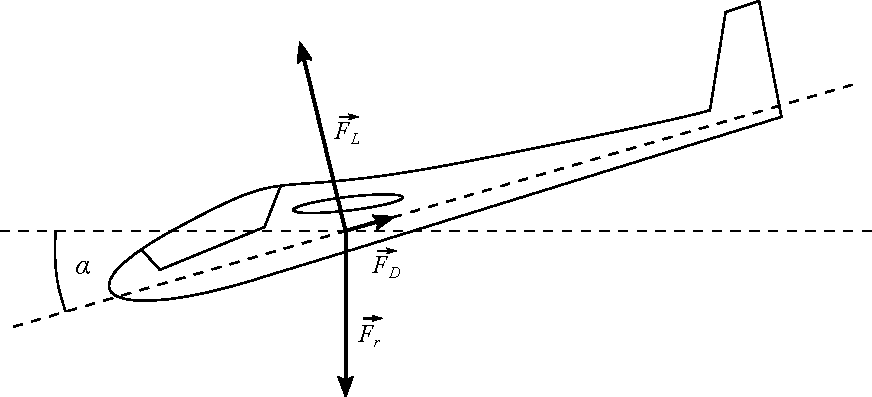
\includegraphics[width=0.7\textwidth]{2020-v2g-05-sol.pdf}
\end{center}


Vaatleme purilennukile mõjuvaid jõude pukseerimise ajal ja vabal liuglemisel. Pukseerimise ajal mõjuvad purilennukile horisontaalselt puksiirköie tõmbejõud $T$ ning õhutakistus $F_D$ ja vertikaalselt raskusjõud $F_r = mg$ ning aerodünaamiline tõstejõud $F_L$. Ühtlase kiirusega lendamisel on purilennukile mõjuvate jõudude (vektoriaalne) summa 0, millest $F_D = T$ ja $F_L = mg$. Seega on purilennuki aerodünaamilisi omadusi iseloomustav suhe antud juhul avaldatav kui
\begin{equation}
	\frac{F_L}{F_D} = \frac{mg}{T}.
\end{equation}

Vabal liuglemisel moodustab lennuki kiirusvektor horisontaalsihi suhtes nurga $\alpha$ ja antud olukorras lennukile mõjuvad jõud on kujutatud joonisel.


Kuna lennuki kiirus on ka sel juhul ühtlane, siis peab jällegi kehtima jõudude tasakaal ehk kõigi kolme jõu vektoriaalne summa on 0. Jõudude horisontaalkomponentide tasakaalust saame $F_L\sin(\alpha) = F_D\cos(\alpha)$, millest:
\begin{equation}
	\frac{F_D}{F_L} = \frac{\sin(\alpha)}{\cos(\alpha)}=\tan(\alpha).
\end{equation}
Märkus: jõudude $F_L$ ja $F_D$ absoluttväärtused on pukseerimisel ja liuglemisel mõnevõrra erinevad, kuid nende suhe $F_D/F_L$ on mõlemal juhul sama.
Viimaks paneme tähele, et kuna purilennuki kiirusvektor moodustab horisontaalsihiga nurga $\alpha$, siis saame maksimaalse lennukauguse $s$ leida täisnurksest kolmnurgast kaatetitega $s$ ja $h$ ning alusnurgaga $\alpha$ ehk $h/s = \tan{\alpha}$. Eelnevalt leitud seoseid kasutades saame
\begin{equation}
s = \frac{h}{\tan(\alpha)} = \frac{hF_L}{F_D} = \frac{hmg}{T},
\end{equation}
mille arvväärtus on $s = \SI{82}{km}$.
\probend